% !TeX root = surprises.tex


\chapter{Construction of a Regular Heptadecagon}\label{c.heptadecagon}

%%%%%%%%%%%%%%%%%%%%%%%%%%%%%%%%%%%%%%%%%%%%%%%%%%%%%%%%%%%%%%%

\abstract*{The Greeks knew how to construct  a triangle, a square, a pentagon and a regular polygon with $15$ sides with a straightedge and compass. In 1796 Carl Friedrich Gauss showed how to construct a regular heptadecagon, a regular polygon with $17$ sides. Gauss's proof which is based upon symmetries of roots of polynomials. An elegant direct construction of a regular heptadecagon by James J. Callagy is given. The chapter also shows how constructions for a regular pentagon can be derived using both geometry and trigonometry.}

%%%%%%%%%%%%%%%%%%%%%%%%%%%%%%%%%%%%%%%%%%%%%%%%%%%%%%%%%%%%%%%

The Greeks knew how to construct a triangle, a square, a pentagon and a regular polygon with $15$ sides with a straightedge and compass. Given a regular polygon with $n$ sides, a polygon with $2n$ sides can be constructed by circumscribing the polygon with a circle and bisecting the central angle (Fig.~\ref{f.hept-double}). In 1796, just before his $19$th birthday, Carl Friedrich Gauss\index{Gauss, Carl Friedrich} awoke one morning and by ``concentrated thought'' figured out how to construct a regular \emph{heptadecagon},\index{Heptadecagon} a regular polygon with $17$ sides. This achievement inspired him to become a mathematician.

Section~\ref{s.hept-regular} discusses the relation between the side of a polygon inscribed in a circle and the central angle that it subtends. Section~\ref{s.fundamental} states without proof the Fundamental Theorem of Algebra. Section~\ref{s.roots} presents the \emph{roots of unity}, the roots of the polynomial $x^n-1$, which are central to Gauss's proof. Sections~\ref{s.gauss} and~\ref{s.derivation} present Gauss's proof which is based upon symmetries of roots of polynomials. Gauss derived a \emph{formula} proving that the heptadecagon is constructible, but a geometric construction was not given for almost a century. Section~\ref{s.construction} gives an elegant construction by James J. Callagy\index{Callagy, James J.}. Section~\ref{s.hept-pentagon} shows how constructions of a regular pentagon can be derived using both geometry and trigonometry.

Some of the material is more straightforward if presented using complex numbers. This material is set off in boxes that can be skipped.
\begin{figure}[b]
\begin{center}
\begin{tikzpicture}[scale=.45]
\coordinate (O) at (0,0);
\vertex{O};
\foreach \x/\name/\n/\po in {0/a/A/right,1/b/B/above,2/c/C/left,3/d/D/below left,4/e/E/below right} {
  \coordinate (\name) at ($(O)+(\x*72+18:3cm)$);
}
\draw (a) -- (b) -- (c) -- (d) -- (e) -- (a);
\node[draw,circle through=(a)] at (O) {};
\draw (d) -- (O) -- (e);
\draw [very thick,dotted] (O) -- (-90:3) -- (e) -- (-90:3) -- (d);
\end{tikzpicture}
\end{center}
\caption{Constructing a regular polynomial with $10$ sides from a regular pentagon}\label{f.hept-double}
\end{figure}

\section{Construction of Regular Polygons}\label{s.hept-regular}

The construction of the regular heptadecagon led to the Gauss-Wantzel theorem\index{Gauss-Wantzel theorem}, which states that a regular polygon with $n$ sides can be constructed with a straightedge and compass if and only if $n$ is the product of a power of $2$ and zero or more \emph{distinct} Fermat numbers\index{Fermat numbers} $2^{2^k}+1$ which are prime. The known Fermat primes are:
\[
F_0=3,\quad F_1=5,\quad F_2=17,\quad F_3=257,\quad F_4=65537\,.
\]
A regular polygon with $257$ sides was constructed by Magnus Georg Paucker\index{Paucker, Magnus Georg} in $1822$ and by Friedrich Julius Richelot $1832$.\index{Richelot, Friedrich Julius} In $1894$ Johann Gustav Hermes\index{Hermes, Johann Gustav} claimed to have constructed a regular polygon  with $65537$ sides.

To construct a regular polygon it is sufficient to construct a line segment of length $\cos \theta$, where $\theta$ is the central angle subtended by a chord that is a side of the polygon inscribed in a unit circle.\index{Regular polygon!cosine of the central angle} Given the line segment $\overline{OB}=\cos\theta$ construct a perpendicular at $B$ and label its intersection with the unit circle by $C$. Then:
\begin{eqnarray*}
\cos \theta&=&\displaystyle\frac{\overline{OB}}{\overline{OC}}=\overline{OB}\\
\theta &=& \cos^{-1} (\overline{OB})\,.
\end{eqnarray*}
The chord $\overline{AC}$ is a side of the regular polygon (Fig.~\ref{f.hept-central1}).
\begin{figure}[b]
\begin{center}
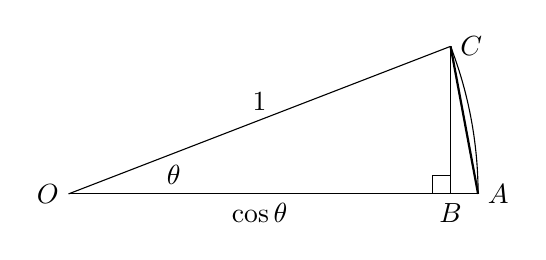
\begin{tikzpicture}[scale=1.3]
\coordinate (O) at (0,0) node[left] {$O$} node[above right,xshift=32pt] {$\theta$};
\coordinate (A) at (4,0);
\node[right] at (A) {$A$};
\draw (O) -- (A);
\draw (A) arc(0:21.12:4);
\coordinate (C) at (21.12:4cm);
\draw (O) -- node[above] {$1$} (C);
\node[right] at (C) {$C$};
\draw (C) -- (C |- A) coordinate (B);
\node[below] at (B) {$B$};
\draw[rotate=90] (B) rectangle +(5pt,5pt);
\draw[thick] (A) -- (C);
\path (O) -- node[below] {$\cos \theta$} (B); 
\end{tikzpicture}
\end{center}
\caption{The cosine of the central angle of a regular polygon}\label{f.hept-central1}
\end{figure}

Given a line segment defined to have length $1$, the lengths that are constructible are those which can be obtained from line segments of known length using the operations $\{+,-,\times,\div,\surd\}$ (Sect.~\ref{s.trisect-constructible}). Gauss showed that the cosine of the central angle of a heptadecagon $360^\circ/17\approx 21.12^\circ$ (Fig.~\ref{f.hept-central4}) is constructible since it can be expressed using only these operations:\index{Heptadecagon!cosine of the central angle}
\begin{eqnarray*}
\cos\left(\frac{360^\circ}{17}\right) &=& 
-\frac{1}{16}+\frac{1}{16}\sqrt{17} + 
     \frac{1}{16}\sqrt{34-2\sqrt{17}}
    + \\
    &&
     \frac{1}{8}\sqrt{
     17+3\sqrt{17} - 
     \sqrt{34-2\sqrt{17}}
   -2
     \sqrt{34+2\sqrt{17}}
   }\,.
\end{eqnarray*}

\begin{figure}[t]
\begin{center}
\begin{tikzpicture}[scale=.8]
\coordinate (O) at (0,0);
\foreach \x/\name in {0/a,1/b,2/c,3/d,4/e,5/f,6/g,7/h,8/i,9/j,10/k,11/l,12/m,13/n,14/o,15/p,16/q} {
  \coordinate (\name) at ($(O)+(\x*21.12:3cm)$);
  \draw (O) -- (\name);
}
\draw (a) -- (b) -- (c) -- (d) -- (e) -- (f) -- (g) -- (h) -- (i) -- (j) -- (k) -- (l) -- (m) -- (n) -- (o) -- (p) -- (q) -- cycle;
\node[above right,xshift=20pt,yshift=-2pt] at (O) {\sm{360^\circ/17\approx 21.12^\circ}};
\draw (O) circle (3cm);
\end{tikzpicture}
\end{center}
\caption{The central angle of a regular heptadecagon}\label{f.hept-central4}
\end{figure}

\section{The Fundamental Theorem of Algebra}\label{s.fundamental}

The following theorem will be used without proof.

\begin{theorem}\label{thm.fundamental} Every polynomial of degree $n$ has exactly $n$ roots.
\end{theorem}\index{Fundamental theorem of algebra}

The statement of the theorem has been simplified because all we will need to know is that $n$ roots \emph{exist}.

\smallskip

\begin{advanced}
\textbf{The Fundamental Theorem of Algebra} states that every non-constant polynomial of degree $n$ in a single variable with \emph{complex} coefficients has exactly $n$ \emph{complex} roots. 
If there are multiple roots with the same value, they are all counted: $x^2-4x+4=(x-2)(x-2)$ has two roots both equal to $2$.
The polynomial $x^2+1$ with integer coefficients has two complex roots $\pm\sqrt{-1}$.
Strangely, even though the theorem is about finite algebraic entities---polynomials of degree $n$ with $n$ roots---methods of analysis, usually complex analysis, are needed to prove the theorem.
\end{advanced}

\section{Roots of Unity}\label{s.roots}

By the Fundamental Theorem of Algebra\index{Fundamental theorem of algebra} (Thm.~\ref{thm.fundamental}) the polynomial $x^{n}-1$ has $n$ roots for any integer $n> 1$. One root is $x=1$ so there are $n-1$ other roots. Denote one of these roots by $r$. Since $r^{n}=1$ it is called an \emph{$n$-th root of unity}.\index{Roots!unity@of unity} What about $r^2$?
\[
(r^{2})^n=(r^{n})^2=1^2=1\,.
\]
It follows that the $n$ numbers:
\[
1, r, r^2, \ldots, r^{n-2}, r^{n-1}
\]
are $n$-th roots of unity.

\begin{advanced}
Let $r$ be $\cos \left(\frac{2\pi}{n}\right) + i\sin  \left(\frac{2\pi}{n}\right)$.
By 	de Moivre's formula:\index{de Moivre's formula}
\[
\left[\cos \left(\frac{2\pi}{n}\right) + i\sin  \left(\frac{2\pi}{n}\right)\right]^{n}=
\cos \left(\frac{2 n\pi}{n}\right) + i\sin  \left(\frac{2 n\pi}{n}\right)= 1\,.
\]
\vspace{-2ex}
\end{advanced}

\begin{theorem}
Let $n$ be a \emph{prime number} and let $r$ an $n$-th root of unity. Then:
\[
\{1,r,r^2,\ldots,r^{n-2},r^{n-1}\}
\]
are distinct so they are \emph{all} the $n$-th roots of unity.
\end{theorem}

\begin{proof}
Suppose that the powers are not distinct so that  $r^i=r^j$ for some $0\leq i<j\leq n-1$. Then $r^j/r^i=r^{j-i}=1$ and there is a positive integer $j\!-\!i<n$ such that $r^{j-i}=1$. Let $m$ be the smallest such positive integer. By the division algorithm for integers, $n=ml+k$ for some $0<l<n$ and $0\leq k<m$. From:
\[
1=r^n=r^{ml+k}=(r^m)^l\cdot r^k=1^l\cdot r^k=r^k\,,
\]
we have $0\leq k<m$ and $r^k=1$. Since $m$  was defined to be the smallest such positive integer $k=0$ and $n=ml$ is not prime.
\end{proof}

\begin{theorem} Let $\{a_1,a_2,\ldots,a_{n-1},a_n\}$ be the roots of an $n$-th degree polynomial $f(x)$. Then:
\begin{align}\label{eq.viete}
f(x) =(x-a_1) (x-a_2)\cdots (x-a_{n-1})(x-a_n)\,.
\end{align}
\end{theorem}

\newpage

\begin{proof}
If $a_i$ is a root of $f(x)$, by definition $f(a_i)=0$, but:
\begin{eqnarray*}
f(a_i)&=&(a_i-a_1) (a_i-a_2)\cdots (a_i-a_{n-1})(a_i-a_n)\\
&=&\cdots (a_i-a_i) \cdots =0\,.
\end{eqnarray*}
Therefore, $f(x)=(x-a_i)g_i(x)$ for some $g_i(x)$ and by induction this holds for all the roots.
\end{proof}

From Eq.~\ref{eq.viete} it is easy to see that the coefficient of $x^{n-1}$ is:
\[
-(a_1+a_2+\cdots+a_{n-1}+a_n)\,.
\]
Since the coefficient of $x^{n-1}$ in $x^n-1$ for $n\geq 2$ is zero, we have:
\begin{eqnarray*}
-(1+r+r^2+\cdots + r^{n-2}+r^{n-1})&=&0\\
r+r^2+\cdots + r^{n-2}+r^{n-1}&=&-1\,.
\end{eqnarray*}
For the heptadecagon this is:
\begin{align}
r+r^2+r^3+r^4+r^5+r^6+r^7+r^8+r^9+r^{10}+r^{11}+r^{12}+r^{13}+r^{14} + r^{15}+r^{16}=-1.\label{eq.minus-one}
\end{align}

\section{Gauss's Proof That a Heptadecagon Is Constructible}\label{s.gauss}

What Gauss understood is that one need not work with the roots in their natural order $r,r^2,\ldots,r^{16}$. The powers of $r^3$ give all these roots but in a different order:
\[
\begin{array}{l}
r^1, \;r^{1\cdot 3 =3},\; r^{3\cdot 3=9},\; r^{9\cdot 3=27=10},\; r^{10\cdot 3=30=13},\; r^{13\cdot 3=39=5},\; r^{5\cdot 3=15},\; r^{15\cdot 3=45=11},\\\\
r^{11\cdot 3 =33=16}, \;r^{16\cdot 3=48=14},\; r^{14\cdot 3=42=8},\; r^{8\cdot 3=24=7},\;r^{7\cdot 3=21=4},\; r^{4\cdot 3=12},\; r^{12\cdot 3=36=2},\; r^{2\cdot 3=6}\,.
\end{array}
\]
Note that the roots have been reduced modulo $17$:
\[
r^{17m+k}=(r^{17})^m\cdot r^k=1^m\cdot r^k=r^k\,.
\]
Check that the list contains all the roots (except $1$) exactly once:
\begin{align}\label{eq.roots}
r^1, r^3, r^9, r^{10}, r^{13}, r^5, r^{15}, r^{11}, r^{16}, r^{14}, r^8, r^7, r^4, r^{12}, r^2, r^6\,.
\end{align}
Given a monic\index{Monic polynomial} quadratic polynomial whose roots are $a,b$:
\[
y^2+py+q=(y-a)(y-b)=0\,,
\]
we can compute the coefficients $p,q$ from the roots (Chap.~\ref{c.quadratic}):
\[
p=-(a+b)\,,\quad q=ab\,.
\]
Therefore, \emph{given} $a+b$ and $ab$, we can write down the \emph{quadratic equation} of which $a,b$ are the roots.

Let $a_0$ be the sum of the roots in the odd positions in Eq.~\ref{eq.roots}:
\[
a_0=r + r^9 + r^{13} +r^{15} +r^{16} + r^8+r^4+r^2\,,
\]
and let $a_1$ be the sum of the roots in the even positions  in Eq.~\ref{eq.roots}:
\[
a_1=r^3 + r^{10} + r^{5} +r^{11} +r^{14} + r^7+r^{12}+r^6\,.
\]
To obtain $a_0,a_1$ as roots of a quadratic equation first compute their sum and use Eq.~\ref{eq.minus-one}:
\[
a_0+a_1=r + r^2 + \cdots +r^{16}=-1\,.
\]
Now we have to work very hard to compute their product. Figure~\ref{fig.a0a1} shows the computation where the values of $r^ir^j$ are written after reducing the exponents modulo $17$. Check that each root occurs exactly four times so that---again using Eq.~\ref{eq.minus-one}---the value of the product is $-4$.
\begin{figure}[t]
\[
\renewcommand{\arraystretch}{1.8}
\begin{array}{lcl}
a_0a_1&=&(r + r^9 + r^{13} +r^{15} +r^{16} + r^8+r^4+r^2)\;\;\times\\
&&(r^3 + r^{10} + r^{5} +r^{11} +r^{14} + r^7+r^{12}+r^6)\\
&=&\occ{4}{1} + \occ{11}{1} + \occ{6}{1} + \occ{12}{1} + \occ{15}{1} + \occ{8}{1} + \occ{13}{1} + \occ{7}{1} +\\
&&\occ{12}{2} + \occ{2}{1} + \occ{14}{1} + \occ{3}{1} + \occ{6}{2} + \occ{16}{1} + \occ{4}{2} + \occ{15}{2} +\\
&&\occ{16}{2} + \occ{6}{3} + \occ{1}{1} + \occ{7}{2} + \occ{10}{1} + \occ{3}{2} + \occ{8}{2} + \occ{2}{2}\;\;\: +\\
&&\occ{1}{2} + \occ{8}{3} + \occ{3}{3} + \occ{9}{1} + \occ{12}{3} + \occ{5}{1} + \occ{10}{2} + \occ{4}{3}\;\;\: +\\
&&\occ{2}{3} + \occ{9}{2} + \occ{4}{4} + \occ{10}{3} + \occ{13}{2} + \occ{6}{4} + \occ{11}{2} + \occ{5}{2} \:+\\
&&\occ{11}{3} + \occ{1}{3} + \occ{13}{3} + \occ{2}{4} + \occ{5}{3} + \occ{15}{3} + \occ{3}{4} + \occ{14}{2} \;+\\
&&\occ{7}{3} + \occ{14}{3} + \occ{9}{3} + \occ{15}{4} + \occ{1}{4} + \occ{11}{4} + \occ{16}{3} + \occ{10}{4} +\\
&&\occ{5}{4} + \occ{12}{4} + \occ{7}{4} + \occ{13}{4} + \occ{16}{4} + \occ{9}{4} + \occ{14}{4} + \occ{8}{4}\\
&=&-4\,.
\end{array}
\]
\caption{Computation of $a_0a_1$. Below each root is its number of occurrences so far.}\label{fig.a0a1}
\end{figure}

Since $a_0+a_1=-1$ and $a_0 a_1=-4$, $a_1,a_2$ are the roots of the quadratic equation $y^2+y-4=0$ and they can be computed using the simple formula for the roots of a quadratic equation:
\[
a_{0,1} = \frac{-1\pm\sqrt{17}}{2}\,.
\]
Let $b_0,b_1,b_2,b_3$ be the sums of every fourth root starting from $r^1,r^3,r^9,r^{10}$, respectively:
\begin{eqnarray*}
b_0&=& r^1+ r^{13} + r^{16} + r^4\\
b_1&=& r^3+ r^{5} + r^{14} + r^{12}\\
b_2&=& r^9+ r^{15} + r^{8} + r^2\\
b_3&=& r^{10}+ r^{11} + r^{7} + r^6\,.
\end{eqnarray*}
Check that $b_0+b_2=a_0, b_1+b_3=a_1$ and compute the corresponding products:
\begin{eqnarray*}
b_0b_2&=&(r + r^{13} + r^{16} +r^4)\;\times\;(r^9 + r^{15} + r^{8} +r^{2})\\
&=&(r^{10}+r^{16}+r^9+r^3)\;+\;(r^{5}+r^{11}+r^4+r^{15})+\\
&&(r^{8}+r^{14}+r^7+r^1)\;+\;(r^{13}+r^{2}+r^{12}+r^6)\\
&=&-1\,,
\end{eqnarray*}
and:
\begin{eqnarray*}
b_1b_3&=&(r^3 + r^{5} + r^{14} +r^{12})\;\times\;(r^{10} + r^{11} + r^{7} +r^{6})\\
&=&(r^{13}+r^{14}+r^{10}+r^9)\;+\;(r^{15}+r^{16}+r^{12}+r^{11})+\\
&&(r^{7}+r^{8}+r^4+r^3)\;+(r^{5}+r^{6}+r^{2}+r^1)\\
&=&-1\,.
\end{eqnarray*}
To summarize these computations:
\begin{eqnarray*}
b_0+b_2&=&a_0\\
b_0b_2&=&-1\\
b_1+b_3&=&a_1\\
b_1b_3&=&-1\,,
\end{eqnarray*}
so $b_0,b_2$ are the solutions of $y^2-a_0y-1= 0$, and $b_1,b_3$ are the solutions of $y^2-a_1y-1 =0$. Using the values previously computed for $a_0,a_1$ we can compute the roots $b_0,b_1$ (Fig.~\ref{f.b0b1}).
\begin{figure}[t]
\begin{eqnarray*}
b_0&=&\frac{a_0+\sqrt{a_0^2+4}}{2}\\
&=&\frac{
     \displaystyle\frac{(-1+\sqrt{17})}{2} + 
     \sqrt{\left(\displaystyle\frac{(-1+\sqrt{17})}{2}\right)^2+4}
   }{2}\\
&=&\frac{
     (-1+\sqrt{17}) + 
     \sqrt{\left(-1+\sqrt{17}\right)^2+16}
   }{4}\\
&=&\frac{
     (-1+\sqrt{17}) + 
     \sqrt{34-2\sqrt{17}}
   }{4}\\
b_1&=&\frac{a_1+\sqrt{a_1^2+4}}{2}\\
&=&\frac{
     \displaystyle\frac{(-1-\sqrt{17})}{2} + 
     \sqrt{\left(\displaystyle\frac{(-1-\sqrt{17})}{2}\right)^2+4}
   }{2}\\
&=&\frac{
     (-1-\sqrt{17}) + 
     \sqrt{\left(-1-\sqrt{17}\right)^2+16}
   }{4}\\
&=&\frac{
     (-1-\sqrt{17}) + 
     \sqrt{34+2\sqrt{17}}
   }{4}\,.
\end{eqnarray*}
\caption{Computation of $b_0$ and $b_1$}\label{f.b0b1}
\end{figure}

\newpage

Finally, let $c_0,c_4$ be the sums of every eighth root starting with $r^1,r^{13}$:
\begin{eqnarray*}
c_0&=&r^1+r^{16}\\
c_4&=&r^{13}+r^4\\
c_0+c_4&=&r^1+r^{16}+r^{13}+r^4=b_0\\
c_0c_4&=&(r^1+r^{16})\cdot(r^{13}+r^4)\\
&=&r^{14}+r^5+r^{12}+r^3=b_1\,,
\end{eqnarray*}
so $c_0,c_4$ are the roots of $y^2-b_0y+b_1=0$. It suffices to compute the root $c_0=r^1+r^{16}$ (Fig.~\ref{fig.c0}).
\begin{figure}[t]
\begin{eqnarray*}
c_0&=&\frac{b_0+\sqrt{b_0^2-4b_1}}{2}\\
&=&\frac{1}{2}
     \frac{
     (-1+\sqrt{17}) + 
     \sqrt{34-2\sqrt{17}}
   }{4}\,+ \\
&& 
    \frac{1}{2}
       \sqrt{\left(\frac{
     (-1+\sqrt{17}) + 
     \sqrt{34-2\sqrt{17}}
   }{4}\right)^2-4\left(\frac{
     (-1-\sqrt{17}) + 
     \sqrt{34+2\sqrt{17}}
   }{4}\right)}
   \\
&=&-\frac{1}{8}+\frac{1}{8}\sqrt{17} + 
     \frac{1}{8}\sqrt{34-2\sqrt{17}}
    + \\
   &&
     \frac{1}{8}\sqrt{
     \left(
     (-1+\sqrt{17}) + 
     \sqrt{34-2\sqrt{17}}
   \right)^2-16\left(
     (-1-\sqrt{17}) + 
     \sqrt{34+2\sqrt{17}}
   \right)}
\\
&=&-\frac{1}{8}+\frac{1}{8}\sqrt{17} + 
     \frac{1}{8}\sqrt{34-2\sqrt{17}}
   \, + \\
   &&
     \frac{1}{8}\sqrt{
     (-1+\sqrt{17})^2 + 
     2(-1+\sqrt{17})\sqrt{34-2\sqrt{17}}+
     (34-2\sqrt{17})
   -}\\
   &&\overline{
     \left((-16-16\sqrt{17}) + 
     16\sqrt{34+2\sqrt{17}}\right)
   }
\\
&=&-\frac{1}{8}+\frac{1}{8}\sqrt{17} + 
     \frac{1}{8}\sqrt{34-2\sqrt{17}}
    \,+ \\
   &&
     \frac{1}{8}\sqrt{
     68+12\sqrt{17} + 
     2(-1+\sqrt{17})\sqrt{34-2\sqrt{17}}
   -16
     \sqrt{34+2\sqrt{17}}
   }
\end{eqnarray*}
\caption{Computation of $c_0$}\label{fig.c0}
\end{figure}

\begin{figure}[b]
\begin{center}
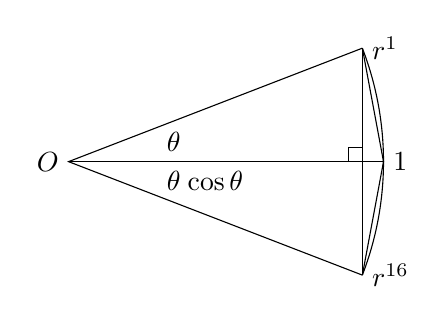
\begin{tikzpicture}[scale=1]
\coordinate (O) at (0,0) node[left] {$O$} node[above right,xshift=32pt] {$\theta$} node[below right,xshift=32pt] {$\theta$};
\coordinate (A) at (4,0);
\node[right] at (A) {$1$};
\draw (O) -- (A);
\coordinate (C) at (21.12:4cm);
\coordinate (D) at (-21.12:4cm);
\draw (D) arc(-21.12:21.12:4);
\draw (D) -- (O) -- (C);
\node[right] at (C) {$r^1$};
\node[right] at (D) {$r^{16}$};
\draw (C) -- (C |- A) coordinate (B);
\draw (D) -- (D |- A);
\draw[rotate=90] (B) rectangle +(5pt,5pt);
\draw (D) -- (A) -- (C);
\path (O) -- node[below] {$\cos \theta$} (B);
\end{tikzpicture}
\end{center}
\caption{The cosine of the central angle computed from $r_1,r_{16}$}\label{f.hept-cosine}
\end{figure}

\clearpage

Therefore, the cosine of the central angle of a heptadecagon is constructible with a straightedge and compass, since it is composed only of rational numbers and the operations $\{+,-,\times,\div,\surd\}$:
\begin{flalign}
\cos\left(\frac{360^\circ}{17}\right) &= 
\frac{c_0}{2}\\
&=-\frac{1}{16}+\frac{1}{16}\sqrt{17} + 
     \frac{1}{16}\sqrt{34-2\sqrt{17}}\; +
    \label{eq.not-gauss1}\\
 & \quad\frac{1}{16}\sqrt{
     68+12\sqrt{17} + 
     2(-1+\sqrt{17})\sqrt{34-2\sqrt{17}}
   -16
     \sqrt{34+2\sqrt{17}}
   }\,.\label{eq.not-gauss2}
\end{flalign}

\begin{advanced}
\vspace{-4ex}
\begin{eqnarray*}
c_0&=&r_1+r_{16}\\
&=&\cos\left(\frac{2\pi}{17}\right)+i\sin\left(\frac{2\pi}{17}\right)+\cos\left(\frac{2\cdot 16\pi}{17}\right)+i\sin\left(\frac{2\cdot 16\pi}{17}\right)\\
&=&\cos\left(\frac{2\pi}{17}\right)+i\sin\left(\frac{2\pi}{17}\right)+\cos\left(\frac{-2\pi}{17}\right)+i\sin\left(\frac{-2\pi}{17}\right)\\
&=&2\cos\left(\frac{2\pi}{17}\right)\,.
\end{eqnarray*}
\vspace{-4ex}
\end{advanced}

\section{Derivation of Gauss's Formula}\label{s.derivation}

The above formula for $\cos(360^\circ /17)$ is not the one given by Gauss. Here is a derivation of Gauss's formula:
\begin{proof}
Let us simplify $2(-1+\sqrt{17})\sqrt{34-2\sqrt{17}}$:
%
\begin{eqnarray*}
2(-1+\sqrt{17})\sqrt{34-2\sqrt{17}} &=&
-2\sqrt{34-2\sqrt{17}} +2\sqrt{17}\sqrt{34-2\sqrt{17}}\\
&&+4\sqrt{34-2\sqrt{17}}-4\sqrt{34-2\sqrt{17}}\\
&=&
2\sqrt{34-2\sqrt{17}} +2\sqrt{17}\sqrt{34-2\sqrt{17}}\\
&&-4\sqrt{34-2\sqrt{17}}\\
&=&2(1+\sqrt{17})\sqrt{34-2\sqrt{17}}-4\sqrt{34-2\sqrt{17}}\,.
\end{eqnarray*}

\newpage

We will remember the term $-4\sqrt{34-2\sqrt{17}}$ for now and simplify the first term by squaring it and then taking the square root:
\begin{eqnarray*}
2(1+\sqrt{17})\sqrt{34-2\sqrt{17}}&=&
2\sqrt{\left[(1+\sqrt{17})\sqrt{34-2\sqrt{17}}\right]^2}\\
&=&2\sqrt{(18+2\sqrt{17})(34-2\sqrt{17})}\\
&=&2\sqrt{(18\cdot 34-4\cdot17)+\sqrt{17}(2\cdot 34 - 2\cdot 18)}\\
&=&2\cdot 4\sqrt{34+2\sqrt{17}}\,.
\end{eqnarray*}
Substituting terms results in Gauss's formula:
\begin{eqnarray*}
\cos\left(\frac{360^\circ}{17}\right) &=&
-\frac{1}{16}+\frac{1}{16}\sqrt{17} + 
     \frac{1}{16}\sqrt{34-2\sqrt{17}} \\
    &&
     +\,\frac{1}{16}\sqrt{
     68+12\sqrt{17} + 
     8\sqrt{34+2\sqrt{17}}-4\sqrt{34-2\sqrt{17}}
   -16
     \sqrt{34+2\sqrt{17}}
   }\\
&=&-\frac{1}{16}+\frac{1}{16}\sqrt{17} + 
     \frac{1}{16}\sqrt{34-2\sqrt{17}}\\
&&+\,\frac{1}{8}\sqrt{
     17+3\sqrt{17} - 
     \sqrt{34-2\sqrt{17}}
   -2
     \sqrt{34+2\sqrt{17}}
   }\,.
\end{eqnarray*}
\end{proof}

\section{Construction of a Heptadecagon}\label{s.construction}

\index{Construction!hept@of a regular heptadecagon}
\index{Heptadecagon!construction}
Construct a unit circle centered at  $O$ with perpendicular diameters  $\overline{QP}$ and $\overline{SR}$ (Fig.~\ref{f.hept-construction1}).
\begin{figure}[t]
\begin{center}
\begin{tikzpicture}[scale=1.2]
\clip (-4.3,-1.8) rectangle (4.3,1.9);

\node at (-.2,1.5) {$\cdots$};
\node at (-.2,1.7) {$R$};
\node at (-.2,-1.5) {$\cdots$};
\node at (-.2,-1.7) {$S$};

\coordinate (O) at (0,0);
\draw (O) circle (4cm);
\coordinate (P) at (4,0);
\coordinate (R) at (0,4);
\coordinate (Q) at (-4,0);
\coordinate (S) at (0,-4);
\coordinate (A) at (0,1);
\coordinate (B) at (.78,0);
\coordinate (C) at (-1.28,0);
\draw (P) -- (Q);
\draw (R) -- (S);
\path (O) -- node[left,xshift=2pt,yshift=-4pt] {$\frac{1}{4}$} (A);
\draw (P) -- ($(P)!1.5!(A)$);
\draw (A) -- node[above] {$\frac{\sqrt{17}}{4}$} (P);
\draw (C) -- (A) -- (B);
\foreach \c/\where in {O/below left, P/right, Q/left, R/above, S/below, A/above left, B/below, C/below} {
  \node[\where] at (\c) {$\c$};
}
\draw (O) rectangle(+5pt,+5pt);
\vertex{O};
\node[below right,xshift=8pt,yshift=-4pt] at (A) {\sm{\alpha}};
\node[below right,xshift=-3pt,yshift=-4pt] at (A) {\sm{\alpha}};
\node[below left,xshift=1pt,yshift=-2pt] at (A) {\sm{\beta}};
\node[below left,xshift=-4pt,yshift=4pt] at (A) {\sm{\beta}};
\draw[<->] ($(C)+(0,-16pt)$) -- node[below] {$\frac{1+\sqrt{17}}{16}$} ($(O)+(0,-16pt)$);
\draw[<->] ($(O)+(0,-16pt)$) -- node[below,xshift=4pt] {$
\frac{-1+\sqrt{17}}{16}$} ($(B)+(0,-16pt)$);
\end{tikzpicture}
\end{center}
\caption{Construction of a heptadecagon (1)}\label{f.hept-construction1}
\end{figure}
Construct $A$ so that $\overline{OA}=(1/4)\overline{OR}$. By Pythagoras's Theorem:
\[
\overline{AP}=\sqrt{(1/4)^2+1^2}=\sqrt{17}/4\,.
\]
Let $B$ be the intersection of the internal bisector of $\angle OAP$ and $\overline{OP}$, and let $C$ be the intersection of the external bisector of $\angle OAP$ and $\overline{QO}$. By the internal angle bisector theorem (Thm.~\ref{thm.angle-bisector}):
\begin{eqnarray*}
\frac{\overline{OB}}{\overline{BP}}&=&\frac{\overline{AO}}{\overline{AP}}\\
\frac{\overline{OB}}{1-\overline{OB}}&=&\frac{1/4}{\sqrt{17}/{4}}\\
\overline{OB}&=&\frac{1}{1+\sqrt{17}}=\frac{1}{1+\sqrt{17}}\cdot \frac{1-\sqrt{17}}{1-\sqrt{17}}\\
&=&\frac{-1+\sqrt{17}}{16}\,,
\end{eqnarray*}
and by the external angle bisector theorem (Thm.~\ref{thm.external-angle-bisector}):
\begin{eqnarray*}
\frac{\overline{OC}}{\overline{CP}}&=&\frac{\overline{AO}}{\overline{AP}}\\
\frac{\overline{OC}}{1+\overline{OC}}&=&\frac{1/4}{\sqrt{17}/{4}}\\
\overline{OC}&=&\frac{1}{-1+\sqrt{17}}=\frac{1}{-1+\sqrt{17}}\cdot \frac{1+\sqrt{17}}{1+\sqrt{17}}\\
&=&\frac{1+\sqrt{17}}{16}\,.
\end{eqnarray*}

\newpage

Construct $D$ on $\overline{OP}$ such that $\overline{CD}=\overline{CA}=a$ (Fig.~\ref{f.hept-construction2}). By Pythagoras's Theorem:
\begin{eqnarray*}
\overline{CD}=\overline{CA}&=&\sqrt{\overline{OA}^2+\overline{OC}^2}\\
&=&\sqrt{\left(\frac{1}{4}\right)^2+\left(\frac{1+\sqrt{17}}{16}\right)^2}=\frac{1}{16}\sqrt{16+1+17+2\sqrt{17}}\\
&=&\frac{1}{16}\sqrt{34+2\sqrt{17}}\,.
\end{eqnarray*}


\begin{figure}[t]
\begin{center}
\begin{tikzpicture}[scale=1.2]
\clip (-4.3,-1.8) rectangle (4.3,1.9);
\coordinate (O) at (0,0);
\draw (O) circle (4cm);
\coordinate (P) at (4,0);
\coordinate (R) at (0,4);
\coordinate (Q) at (-4,0);
\coordinate (S) at (0,-4);
\coordinate (A) at (0,1);
\coordinate (B) at (.78,0);
\coordinate (C) at (-1.28,0);

\coordinate (D) at (.344,0);
\coordinate (E) at (2.05,0);
\coordinate (M) at (-1.8275,0);
\coordinate (F) at (0,-1);

\draw (P) -- (Q);
\draw (R) -- (S);
\draw (A) -- (P);
\draw (C) -- node[above] {$a$} (A) -- node[xshift=2pt,right] {$b$} (B);
\path (Q) -- node[below] {$f$}  (M);
\path (B) -- node[below] {$b$} (E);

\path[name path=circ] (M) circle (2.1725cm);
\path[name path=yaxis] (R) -- (S);
\path[name intersections={of=circ and yaxis,by={F1,F}}];
\draw (M) -- node[below] {$f$} (F);

\draw[<->] ($(C)+(0,-9pt)$) -- node[fill=white] {$a$} ($(D)+(0,-9pt)$);

\foreach \c/\where in {O/below left, P/right, Q/left, R/above, S/below, A/above left, B/below, C/below, D/below, E/below, M/below left, F/below left} {
  \node[\where] at (\c) {$\c$};
}
\draw (O) rectangle(+5pt,+5pt);
\vertex{O};
\vertex{E};
\vertex{D};
\end{tikzpicture}
\end{center}
\caption{Construction of a heptadecagon (2)}\label{f.hept-construction2}
\end{figure}


Construct $E$ on $\overline{OP}$ such that $\overline{BE}=\overline{BA}=b$; again by Pythagoras's Theorem:

\begin{eqnarray*}
\overline{BE}=\overline{BA}&=&\sqrt{\overline{OA}^2+\overline{OB}^2}\\
&=&\sqrt{\left(\frac{1}{4}\right)^2+\left(\frac{1-\sqrt{17}}{16}\right)^2}=\frac{1}{16}\sqrt{16+1+17-2\sqrt{17}}\\
&=&\frac{1}{16}\sqrt{34-2\sqrt{17}}\,.
\end{eqnarray*}
Construct $M$ as the midpoint of $\overline{QD}$ and construct $F$ on $\overline{OS}$ such that $\overline{MF}=\overline{MQ}=f$:
%
\begin{eqnarray*}
\overline{MF}=\overline{MQ}&=&\frac{1}{2}\overline{QD}=\frac{1}{2}(\overline{QC}+\overline{CD})=\frac{1}{2}((1-\overline{OC})+\overline{CD})\\
&=&\frac{1}{2}\left[1-\left(\frac{1+\sqrt{17}}{16}\right)+\frac{\sqrt{34+2\sqrt{17}}}{16}\right]\\
&=&\frac{1}{32}\left(15-\sqrt{17}+\sqrt{34+2\sqrt{17}}\right)\,.
\end{eqnarray*}

Construct a circle whose diameter is $\overline{OE}$. Construct a chord $\overline{OG}=\overline{OF}=g$ (Fig.~\ref{f.hept-construction3}). Note that $\overline{MO}=1-\overline{MQ}=1-\overline{MF}$. By Pythagoras's Theorem:
\begin{figure}[b]
\begin{center}
\begin{tikzpicture}[scale=1.2]
\clip (-4.3,-1.8) rectangle (4.3,1.9);
\coordinate (O) at (0,0);
\draw (O) circle (4cm);
\coordinate (P) at (4,0);
\coordinate (R) at (0,4);
\coordinate (Q) at (-4,0);
\coordinate (S) at (0,-4);
\coordinate (A) at (0,1);
\coordinate (B) at (.78,0);
\coordinate (C) at (-1.28,0);

\coordinate (D) at (.5,0);
\coordinate (E) at (2.045,0);
\coordinate (M) at (-1.8275,0);

\path[name path=circ] (M) circle (2.1725cm);
\path[name path=yaxis] (R) -- (S);
\path[name intersections={of=circ and yaxis,by={F1,F}}];
\draw (M) -- node[below] {$f$} (F);

\draw[name path=OEarc] (E) arc(0:-180:1.025cm);
\path[name path=OFcircle] (O)
  let
    \p1 = ($(O)-(F)$)
  in
    circle({veclen(\x1,\y1)});
\path[name intersections={of=OEarc and OFcircle, by={G}}];
\draw (O) -- node[above,near end,xshift=2pt] {$g$} (G) -- node[below] {$e$} (E);
\path (O) -- node[left] {$g$} (F);

\path[name path=EGcircle] (E) 
  let
  \p1 = ($(E)-(G)$)
  in
    circle({veclen(\x1,\y1)});
\draw[name path=PQ] (P) -- (Q);
\path[name intersections={of=PQ and EGcircle, by={H,H1}}];
\path (E) -- node[below] {$e$} (H);

\draw (R) -- (S);
\draw (A) -- (P);
\draw (C) -- (A) -- (B);
\draw (M) -- (F);

\foreach \c/\where in {O/below left, P/right, Q/left, R/above, S/below, A/above left, B/below, C/below, D/below, E/below right, M/below left, F/below left, G/below, H/below} {
  \node[\where] at (\c) {$\c$};
}
\vertex{O};
\vertex{D};

\draw (O) rectangle +(+5pt,+5pt);
\draw[rotate=30] (G) rectangle +(+5pt,+5pt);
\path (Q) -- node[below] {$f$} (M);
\end{tikzpicture}
\end{center}
\caption{Construction of a heptadecagon (3)}\label{f.hept-construction3}
\end{figure}

\begin{eqnarray*}
\overline{OG}=\overline{OF}&=&\sqrt{\overline{MF}^2-\overline{MO}^2}=\sqrt{\overline{MF}^2-(1-\overline{MF})^2}\\
&=&\sqrt{2\overline{MF}-1}\\
&=&\sqrt{\frac{1}{16}\left(15-\sqrt{17}+\sqrt{34+2\sqrt{17}}\right)-1}\\
&=&\frac{1}{4}\sqrt{-1-\sqrt{17}+\sqrt{34+2\sqrt{17}}}\,.
\end{eqnarray*}
$\angle OGE$ is a right angle since it is subtended by a diameter of the circle. Construct $H$ on $\overline{OP}$ such that $\overline{EH}=\overline{EG}=e$; again by Pythagoras's Theorem:
\begin{eqnarray*}
\overline{EH}=\overline{EG}&=&\sqrt{\overline{OE}^2-\overline{OG}^2}=\sqrt{(\overline{OB}+\overline{BE})^2-\overline{OG}^2}\\
&=&\sqrt{\left(\frac{-1+\sqrt{17}}{16}+\frac{\sqrt{34-2\sqrt{17}}}{16}\right)^2-
\frac{1}{16}\left(-1-\sqrt{17}+\sqrt{34+2\sqrt{17}}\right)}
\\
&=&\frac{1}{16}\sqrt{\left(
(18-2\sqrt{17})+ 2(-1+\sqrt{17})\sqrt{34-2\sqrt{17}}+
(34-2\sqrt{17})\right)}\\
&&\quad\quad\quad\overline{
+\left(16+16\sqrt{17}-16\sqrt{34+2\sqrt{17}}\right)}\\
&=&\frac{1}{16}\sqrt{
68+12\sqrt{17}-16\sqrt{34+2\sqrt{17}}-2(1-\sqrt{17})\sqrt{34-2\sqrt{17}}
}\,.
\end{eqnarray*}
Compute $\overline{OE}$:
\begin{eqnarray*}
\overline{OE}=\overline{OB}+\overline{BE}&=&\frac{-1+\sqrt{17}}{16}+\frac{1}{16}\sqrt{34-2\sqrt{17}}\\
&=&\frac{1}{16}\left(-1+\sqrt{17}+\sqrt{34-2\sqrt{17}}\right)\,.
\end{eqnarray*}
Finally, $\overline{OH}=\overline{OE}+\overline{EH}$ which is Gauss's formula for $\cos (360^\circ/17)$.



\section{Construction of a Regular Pentagon}\label{s.hept-pentagon}
\index{Construction!pent@of a regular pentagon}

\begin{advanced}
The complex fifth roots of unity are:
\[
1+i\cdot 0,\quad\frac{\sqrt{5}-1}{4}\pm i \frac{\sqrt{10+2\sqrt{5}}}{4},\quad\frac{-\sqrt{5}-1}{4}\pm i \frac{\sqrt{10-2\sqrt{5}}}{4}\,.
\]
\vspace{-3ex}
\end{advanced}

\subsection{Trigonometry}
The central angle of a regular pentagon is $360^\circ/5=72^\circ$  (Fig.~\ref{f.hept-central-pentagon}). Let us compute $\cos 36^\circ$ using the  trigonometric identities for $2\theta$ and $\theta/2$ (Thms.~\ref{s.sum-of-trig}, \ref{thm.sine-cosine-half}):
\begin{figure}[t]
\begin{center}
\begin{tikzpicture}[scale=.5]
\coordinate (O) at (0,0);
\vertex{O};
\node[below right,xshift=6pt,yshift=2pt] at (O) {$72^\circ$};
\foreach \x/\name/\n/\po in {0/a/A/right,1/b/B/above,2/c/C/left,3/d/D/below left,4/e/E/below right} {
  \coordinate (\name) at ($(O)+(\x*72+18:3cm)$);
}
\draw (a) -- (b) -- (c) -- (d) -- (e) -- (a);
\node[draw,circle through=(a)] at (O) {};
\draw (a) -- (O) -- (e);
\end{tikzpicture}
\end{center}
\caption{The central angle of a regular pentagon}\label{f.hept-central-pentagon}
\end{figure}
\begin{eqnarray*}
0=\cos 90^\circ &=& \cos(72^\circ+18^\circ)=\cos 2\cdot 36^\circ\cos 36^\circ/2 - \sin 2\cdot 36^\circ\sin 36^\circ/2\\
&=&(2\cos^2 36^\circ-1)\sqrt{\frac{1+\cos 36^\circ}{2}}-2\sin 36^\circ\cos 36^\circ\sqrt{\frac{1-\cos 36^\circ}{2}}\,.
\end{eqnarray*}

\newpage

There is now only one angle in the formula; let $x=\cos 36^\circ$. Then:
\begin{eqnarray*}
(2x^2-1)\sqrt{\frac{1+x}{2}}&=&2\sqrt{1-x^2}\cdot x \cdot \sqrt{\frac{1-x}{2}}\\
(2x^2-1)\sqrt{1+x}&=&2\sqrt{1-x}\cdot\sqrt{1+x}\cdot x \cdot \sqrt{1-x}\\
2x^2-1&=&2x(1-x)\\
4x^2-2x-1&=&0\,.
\end{eqnarray*}
Solving the quadratic equation gives a constructible value:
\[
\cos 36^\circ = \frac{1+\sqrt{5}}{4}\,.
\]

%\vspace*{-6ex}

\subsection{Geometry}\label{s.geometry-pentagon}

Let $\overline{ABCDE}$ be a regular pentagon (Fig.~\ref{f.hept-pentagon2}). By definition all the sides and all the interior angles are equal. It is easy to show by congruent triangles that all diagonals are equal. Let the length of the sides be $1$ and the length of the diagonals be $x$.

\begin{figure}[t]
\begin{center}
\begin{tikzpicture}[scale=.8]
\coordinate (O) at (0,0);
\vertex{O};
\node[above left,xshift=1pt,yshift=4pt] at (O) {$O$};
\foreach \x/\name/\n/\po in {0/a/A/right,1/b/B/above,2/c/C/left,3/d/D/below left,4/e/E/below right} {
  \coordinate (\name) at ($(O)+(\x*72+18:3cm)$);
  \node[\po] at (\name) {$\n$};
}
\draw (a) -- node[above] {$1$} (b) -- node[above] {$1$} (c) -- node[left] {$1$} (d) -- node[below] {$1$} (e) -- node[right] {$1$} (a);
\draw[thick] (a) -- node[above] {$x$} (c);
\draw[thick,name path=ad] (a) -- node[above] {$x$} (d);
\draw[thick,name path=cd] (c) -- node[above] {$x$} (e);
\path[name intersections={of=ad and cd,by={f}}];
\node[above] at (f) {$\psi$};
\vertex{f};
\node[below] at (f) {$\psi$};
\node[right,xshift=6pt] at (f) {$F$};
\node[below right,xshift=14pt] at (c) {$\theta$};
\node[below left,xshift=-14pt] at (a) {$\theta$};
\node[above right,xshift=16pt] at (d) {$\phi$};
\node[above left,xshift=-16pt] at (e) {$\phi$};
\end{tikzpicture}
\end{center}
\caption{Construction of a regular pentagon (1)}\label{f.hept-pentagon2}
\end{figure}
$\triangle ACE\cong \triangle CAD$ by side-side-side so $\angle ACE=\angle CAD=\theta$. $\triangle AED\cong\triangle CDE$ by side-side-side so $\angle ADE=\angle CED=\phi$. $\angle AFC=\angle EFD=\psi$ are vertical angles.
$\psi+2\theta=\psi+ 2\phi=180^\circ$ so $\theta=\phi$.
By alternate interior angles, we conclude that $\overline{AC}\parallel \overline{DE}$.
\begin{figure}[t]
\begin{center}
\begin{tikzpicture}[scale=.8]
\coordinate (O) at (0,0);
\vertex{O};
\node[above left,xshift=1pt,yshift=4pt] at (O) {$O$};

\foreach \x/\name/\n/\po in {0/a/A/right,1/b/B/above,2/c/C/left,3/d/D/below left,4/e/E/below right} {
  \coordinate (\name) at ($(O)+(\x*72+18:3cm)$);
  \node[\po] at (\name) {$\n$};
}
\draw (a) -- node[above] {$1$} (b) -- node[above] {$1$} (c) -- node[left] {$1$} (d) -- node[below] {$1$} (e);
\draw[very thick] (e)-- node[right] {$1$} (a);
\draw[very thick] (a) -- (c);
\draw[very thick] (c) -- node[below] {$x$} (e);

\path[name path=ef] (e) -- +(108:5);
\path[name path=ac] (a) -- (c);
\path[name intersections={of=ac and ef,by={f}}];
\vertex{f};
\node[above] at (f) {$F$};
\draw[very thick] (e) -- node[right] {$1$} (f);
\path (a) -- node[above,xshift=-4pt] {$x-1$} (f);
\node[below left] at (a) {$\alpha$};
\node[below right,xshift=2pt] at (f) {$\alpha$};
\path (c) -- node[above] {$1$} (f);
\draw ($(e)+(72:.5)$) arc(72:144:.5cm);
\node[above,yshift=12pt] at (e) {$\alpha$};
\end{tikzpicture}
\end{center}
\caption{Construction of a regular pentagon (2)}\label{f.hept-pentagon3}
\end{figure}

Construct a line through $E$ parallel to $\overline{DC}$ and let $F$ be its intersection with $\overline{AC}$ (Fig.~\ref{f.hept-pentagon3}). $\overline{CDEF}$ is a rhombus so $\overline{EF}=\overline{CD}=\overline{AE}=1$. $\triangle ACE$ is an isoceles triangle with base angles $\alpha$. $\triangle AEF$ is also isoceles and $\angle AFE=\angle FAE=\alpha$. Therefore,$\triangle ACE\sim\triangle AEF$:
\[
\frac{x}{1}=\frac{1}{x-1}\,.
\]
The result is a quadratic equation $x^2-x-1=0$
whose positive root is constructible:
\[
x=\frac{1+\sqrt{5}}{2}\,.
\]

\subsection*{What Is the Surprise?}

It is surprising that two millennia passed from the work of the Greeks on construction to the discovery by Gauss of the constructibility of the regular heptadecagon. It is also surprising that the problem was solved not by using geometry, but by inventing new algebraic methods that had a far-reaching influence in mathematics.


\subsection*{Sources}

This chapter is based on \cite{jorg}. Gauss's original work is available in an English translation \cite{gauss}.
Equation~\ref{eq.not-gauss1}--\ref{eq.not-gauss2} appears in \cite{rike}; the author assigns an exercise to transform it into Gauss's formula that appears in \cite[p.~458]{gauss} and \cite[p.~68]{jorg}.

The construction of the heptadecagon is taken from \cite{callagy} while other constructions can be found in \cite{wiki:heptadecagon}. The trigonometric construction of the regular pentagon is from \cite{wiki:pentagon}. The geometric construction of the regular pentagon was obtained by solving exercises 2.3.3 and 2.3.4 in \cite{stillwell}.
